\documentclass[a4paper,oneside,onecolumn]{article}
\usepackage{graphicx}
\usepackage{amsmath}
\usepackage{amssymb}
\usepackage{subfigure}
\renewcommand{\figurename}{Figure S}
%\usepackage{epstopdf}
\usepackage{setspace}
\onehalfspace
\usepackage{authblk}
\usepackage[margin=2.3cm]{geometry}

%\geometry{a4paper,left=2.3cm,right=2.3cm,top=2.5cm,bottom=4.5cm}
\newcommand{\nm}{\ensuremath{\,\textrm{nm}}}
\newcommand{\eV}{\ensuremath{\,\textrm{eV}}}
\newcommand{\uM}{\ensuremath{\,\mu\textrm{M}}}
\newcommand{\uW}{\ensuremath{\,\mu\textrm{W}}}
\newcommand{\meV}{\ensuremath{\,\textrm{meV}}}

\title{Supplementary information for: In situ tuning of nanorods' plasmon
through oxidative etching with KCN}
\author[1]{Aquiles Carattino}
\author[2]{Saumyakanti Khatua}
\author[1]{Michel Orrit}
\affil[1]{Leiden Institute of Physics, Leiden, The Netherlands}
\affil[2]{Indian Institute of Technology- Gandhinagar, Ahmedabad,  India}
%\ead{Corresponding Author Email Address}
%\cortext[a]{khatuask@iitgn.ac.in, Orrit@physics.leidenuniv.nl }

\begin{document}
\maketitle

\section{Bulk Results}
\begin{figure}[htp]
 \centering
 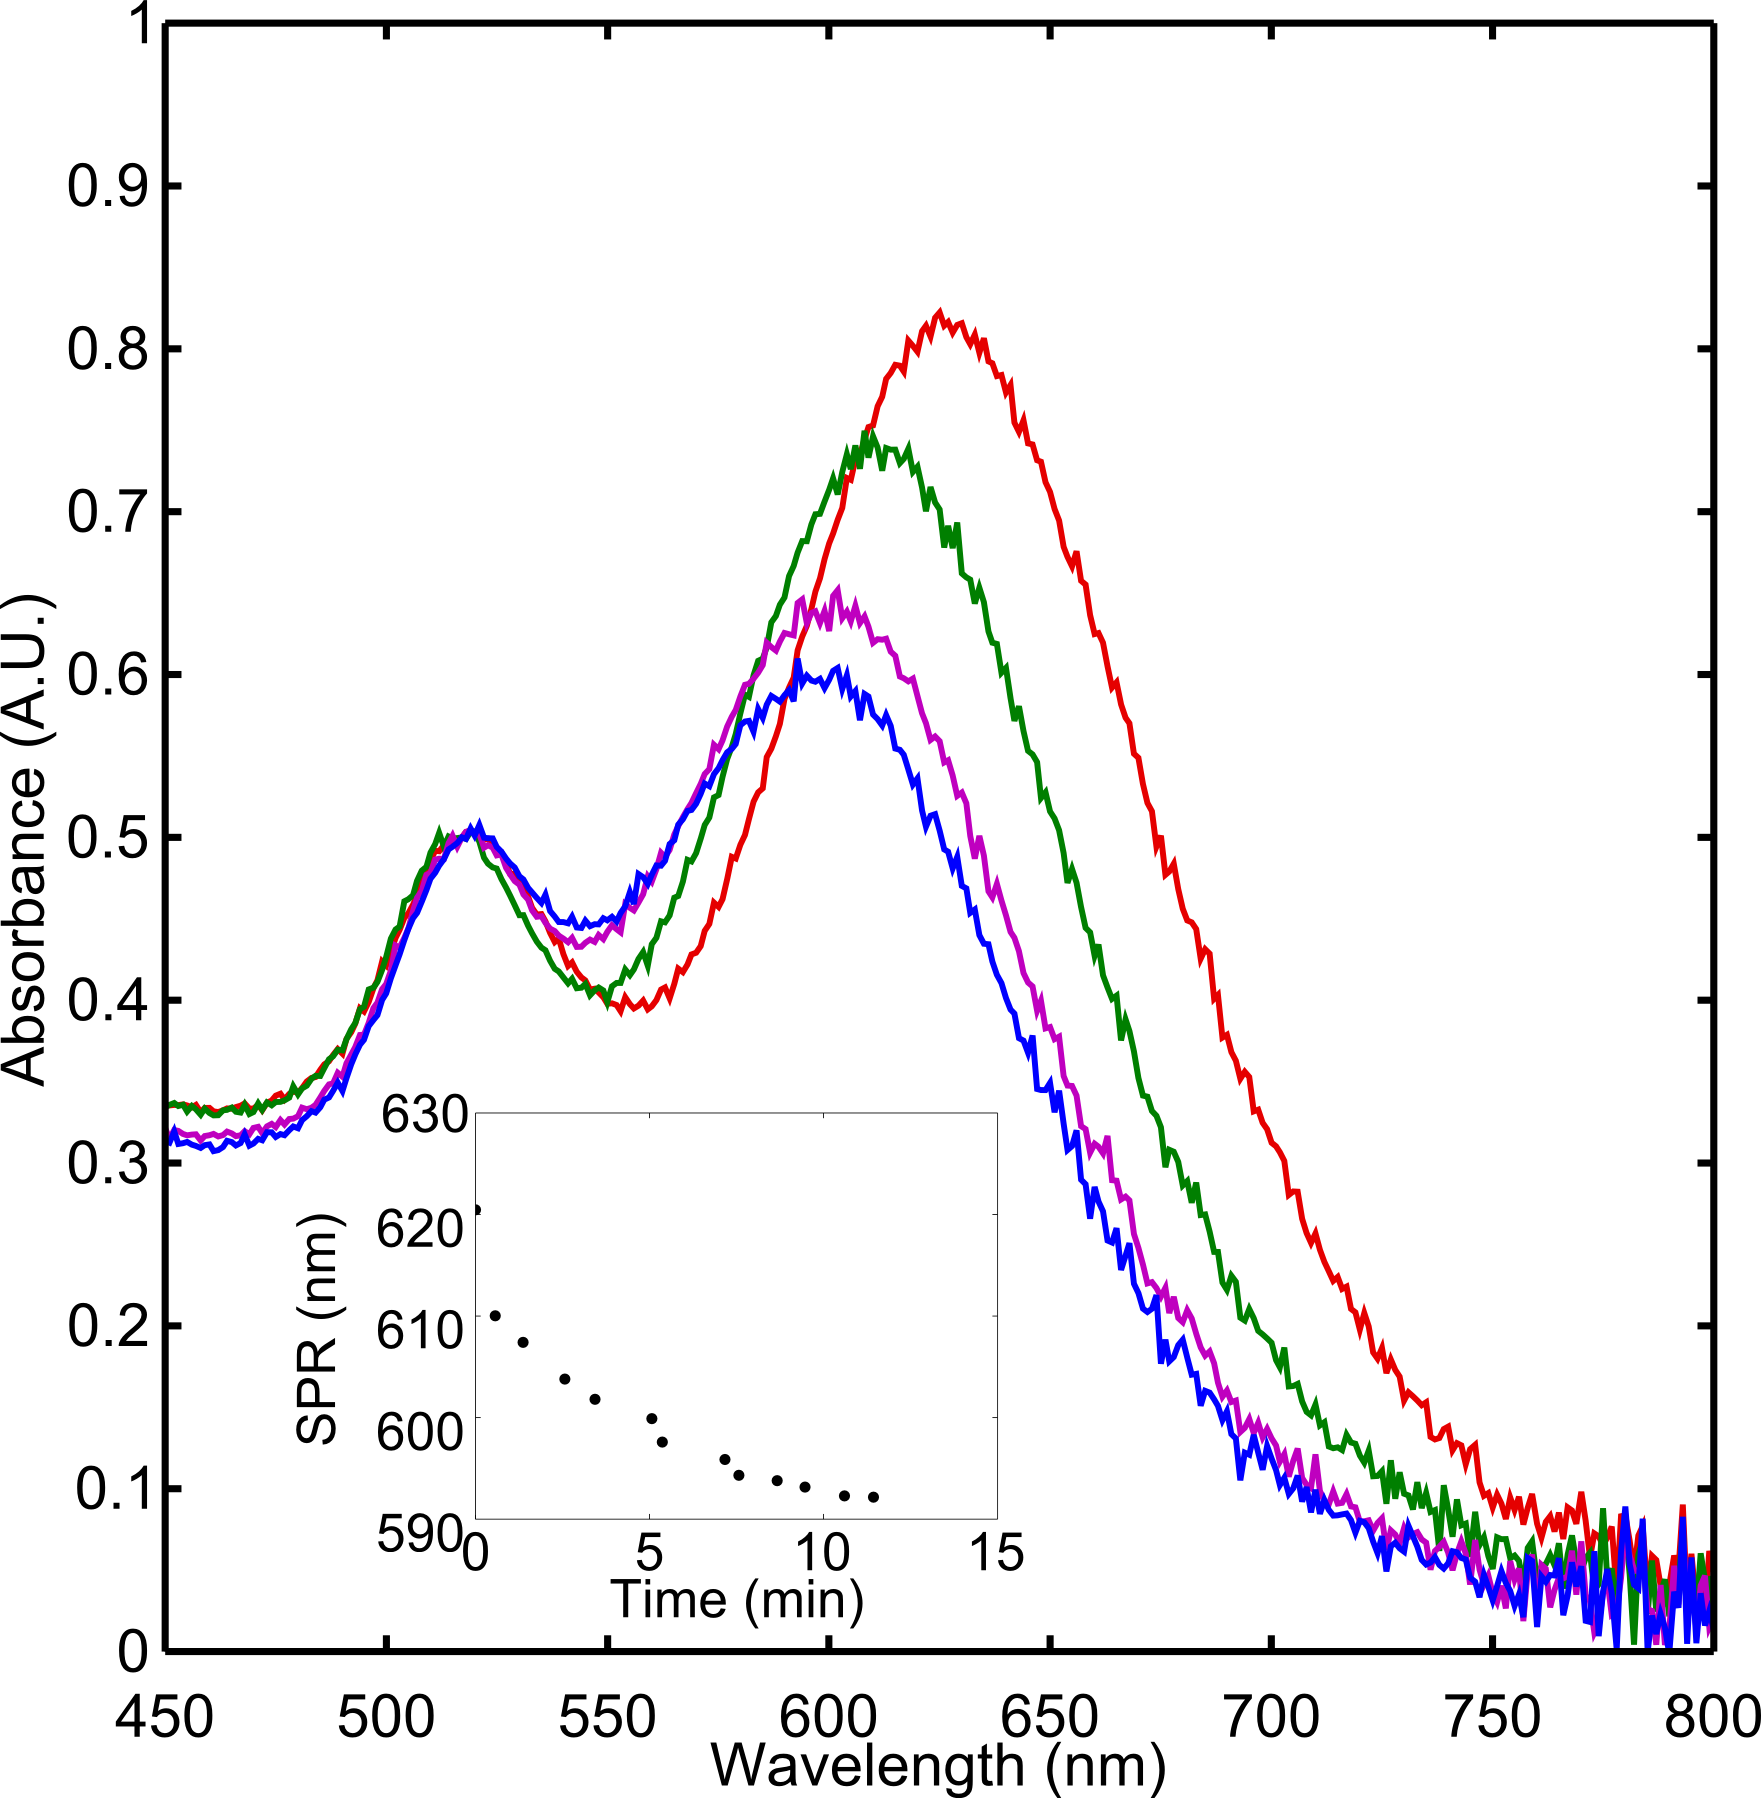
\includegraphics[width=0.45\linewidth]{Figures/04_Supporting/01_Bulk/01_bulk.png}
 \caption{Extinction spectra of a bulk suspension of gold nanorods dispersed in
 $100\uM$ KCN. The curves are displayed at 2 minutes intervals. The
 inset shows the peak position as a function of time. The curves were normalized
 to the transverse peak for clarity.}
 \label{fig:Bulk}
\end{figure}

Figure S\ref{fig:Bulk} shows the behavior of the same nanorods dispersed in
$100\uM$ KCN. It is possible to observe a clear blue shift of the longitudinal
plasmon resonance, towards the transverse peak at around $530\nm$. As stated in
the main text, we attribute the blue shift of the peak to a shortening of the
long axis of the rods. This is because the CTAB is more efficient in protecting
the sides than the tips of the particles. It is also possible to note an asymptotic
blue-shift of the plasmon. We attribute this to a complete reaction of the KCN
with the gold atoms. If more KCN was added to the vial, the blue-shift would
have continued. 

The spectra were acquired in an UV-Vis spectrometer. The first spectrum was
acquired with the rods dispersed in water, before adding KCN into the vial.
Later a solution such that the final concentration was $100\uM$ was added and a
set of automatic spectra was recorded at a fixed interval of time. The peak
position was extracted by fitting a double lorentzian, one with a fixed central
wavelength (the transverse resonance) and a second one for the longitudinal
plasmon.


\section{SEM Images}

\begin{figure}[htp]
 \centering
 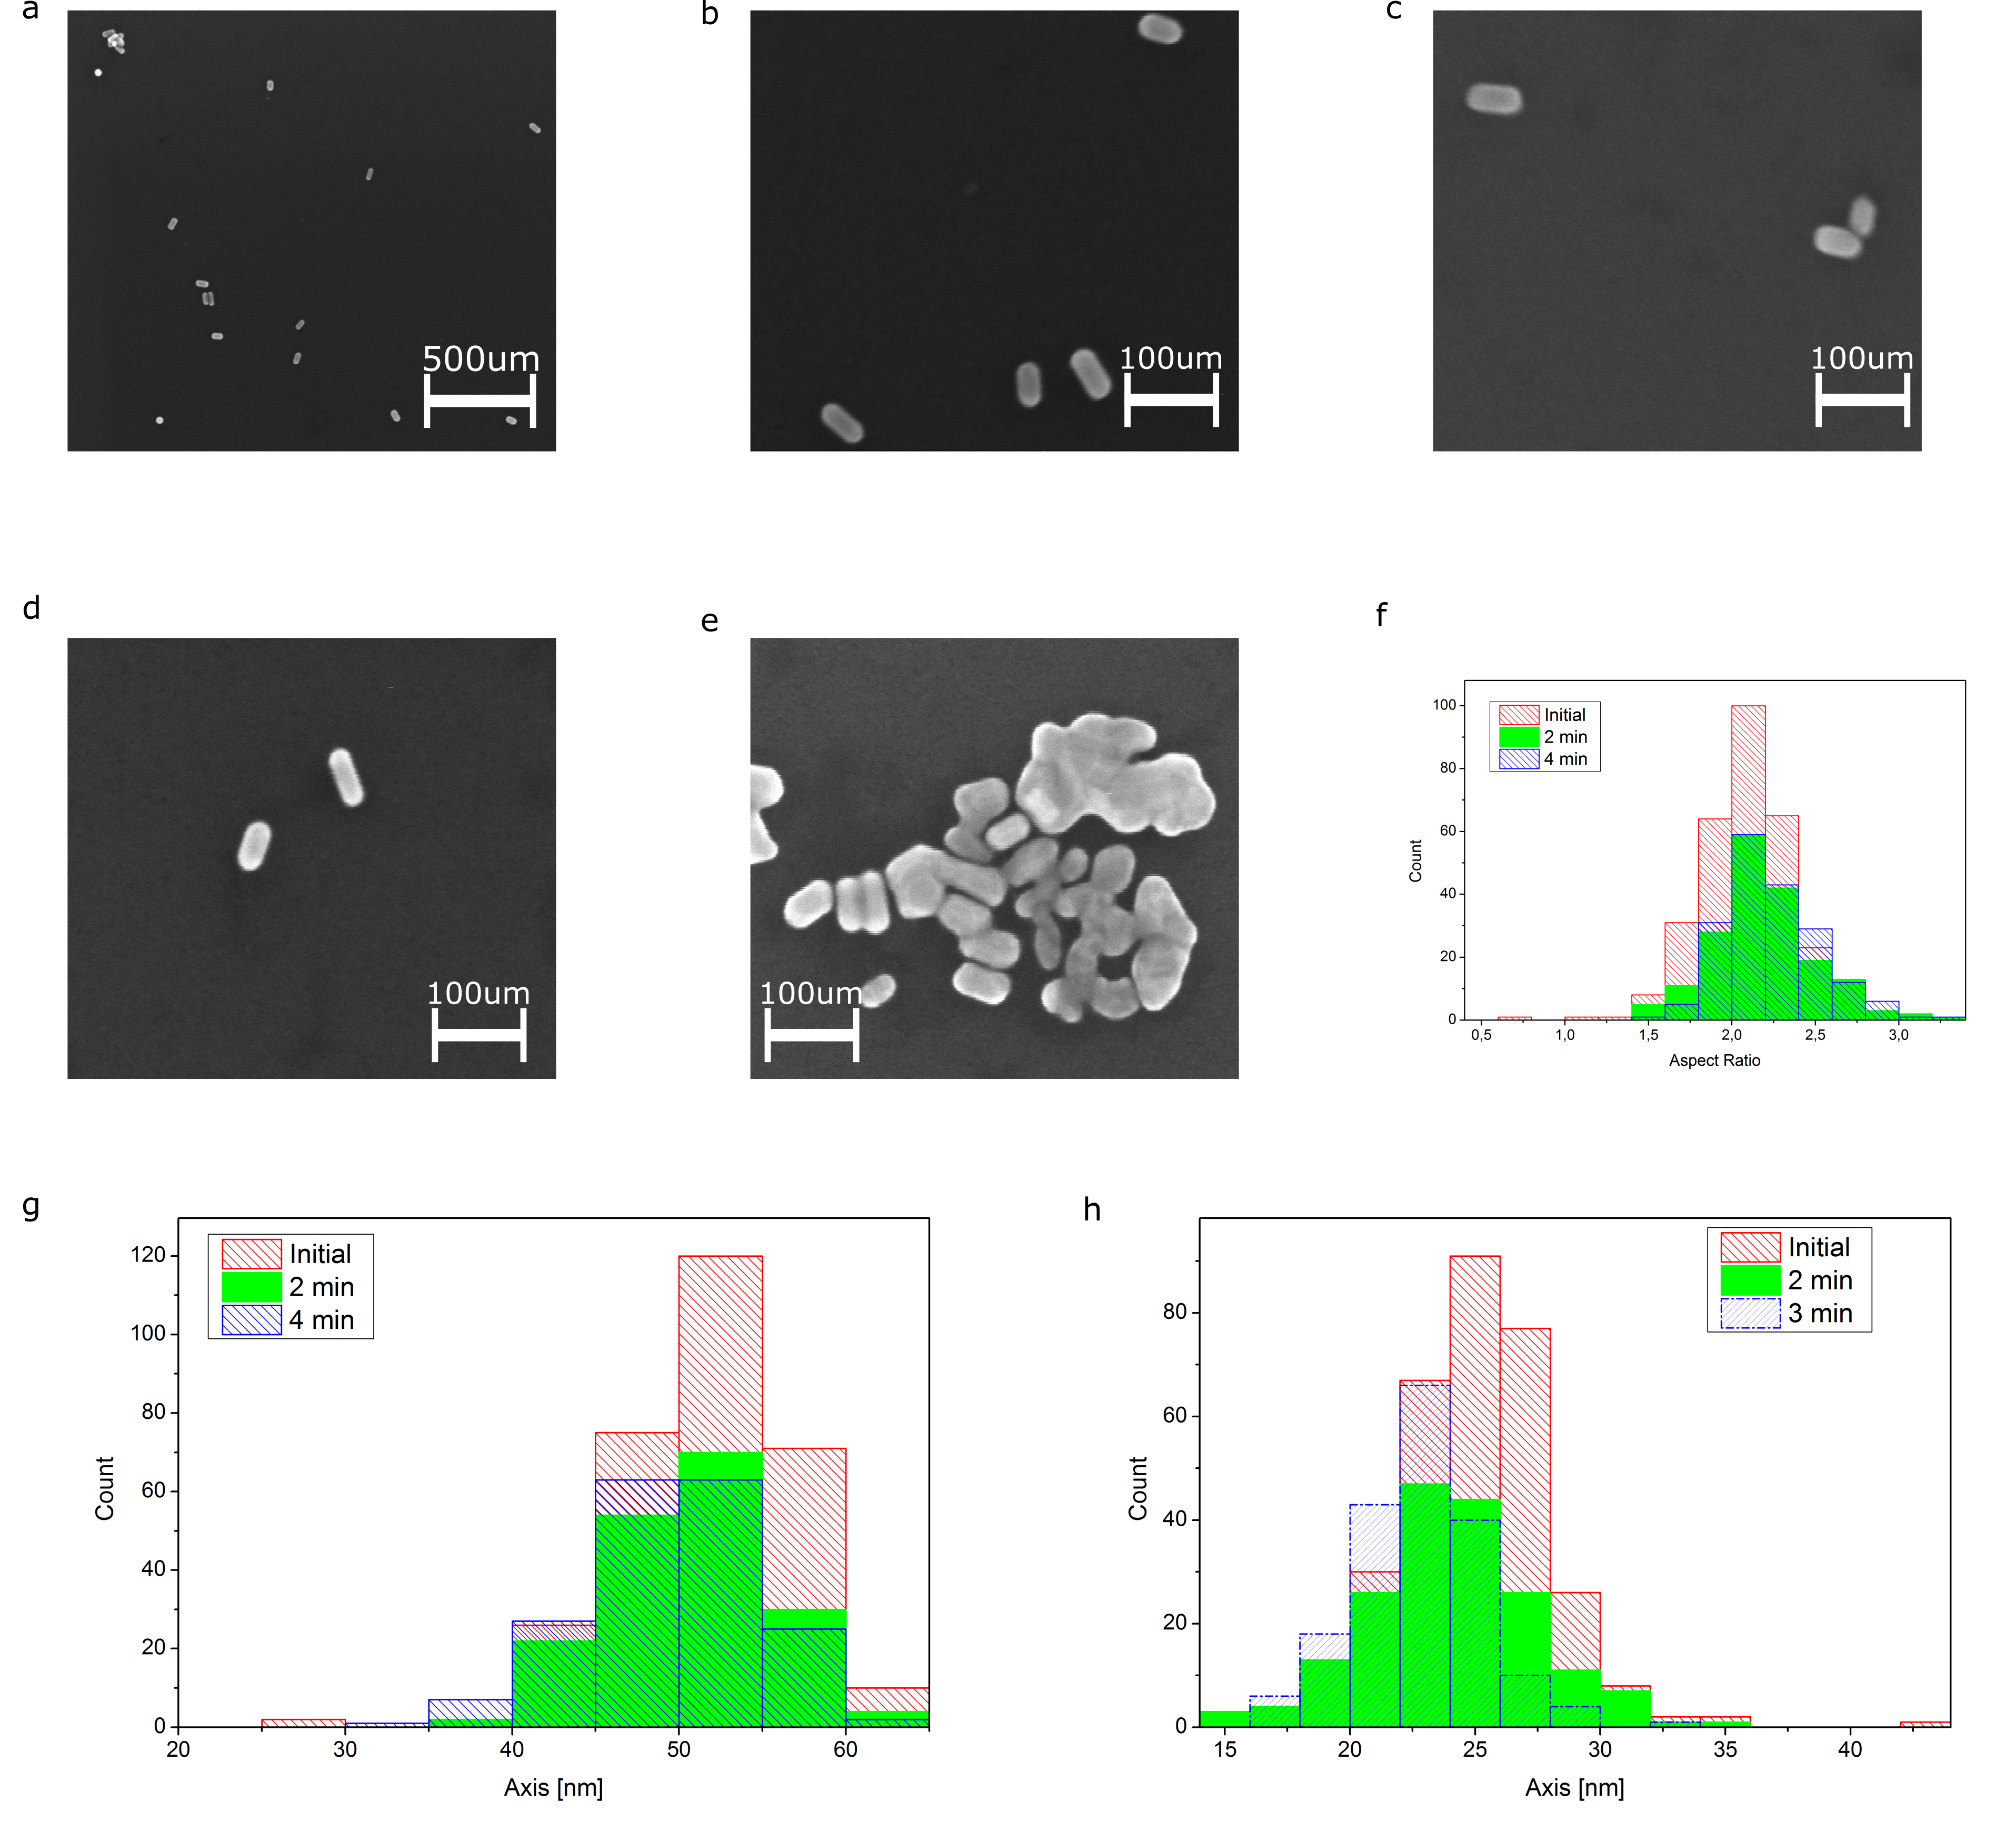
\includegraphics[width=0.95\linewidth]{Figures/04_Supporting/02_SEM/sem.png}
 \caption{SEM Images of the rods a) after synthesis, b) after $2$ minutes in
 $20\uM$ KCN when particles are separated, c) or when they form clusters. d)
 separated particles after $4$ minutes in KCN and e) when they were forming a
 cluster. f-h) Histograms of the aspect ratio (f), longitudinal(g) and
 transverse axis(h) for each of the cases (before, after $2$ and after $4$
 minutes in KCN.) }
 \label{fig:SEM}
\end{figure}

Figure S\ref{fig:SEM} shows the SEM images of the rods. In S\ref{fig:SEM}a an
example of the rods after synthesis and before being etched.
Figures S\ref{fig:SEM}b and S\ref{fig:SEM}c are after $2$ minutes in $20\uM$ KCN
and the difference on the shape of the particles when they are separated from each other and in contact is
notable. Figures S\ref{fig:SEM}d and S\ref{fig:SEM}e were taken after $4$
minutes in KCN.
The histograms in Figures S\ref{fig:SEM}f-h show the analysis of the aspect
ratio, the longitudinal and the transverse axis respectively for each of the  cases. The
changes observed for the axis are inside the standard distribution of each
parameter. Table \ref{tab:SEM_results} summarizes the averaged values found
after analyzing approximately $300$ particles. However the small shift in the
average is consistent with the optical results, yielding an etching rate of
$0.5\,\textrm{nm}/\min$.

\begin{table}[htp]
\begin{tabular*}{0.48\textwidth}{c c c c c}
 $\,$ & L (nm) & Sdv (nm) & R (nm) & Sdv (nm) \\\hline
 $0\textrm{min}$ & $51$ & $5$ & $24$ & $3$ \\ 
 $2\textrm{min}$ & $50$ & $5$ & $23$ & $3$ \\
 $4\textrm{min}$ & $49$ & $5$ & $22$ & $2$ \\
\end{tabular*}
\label{tab:SEM_results}
\caption{Summary of the results obtained for 300 different particles while
imaging them with an SEM.}
\end{table}

\section{Background Spectrum}
\begin{figure}[htp]
 \centering
 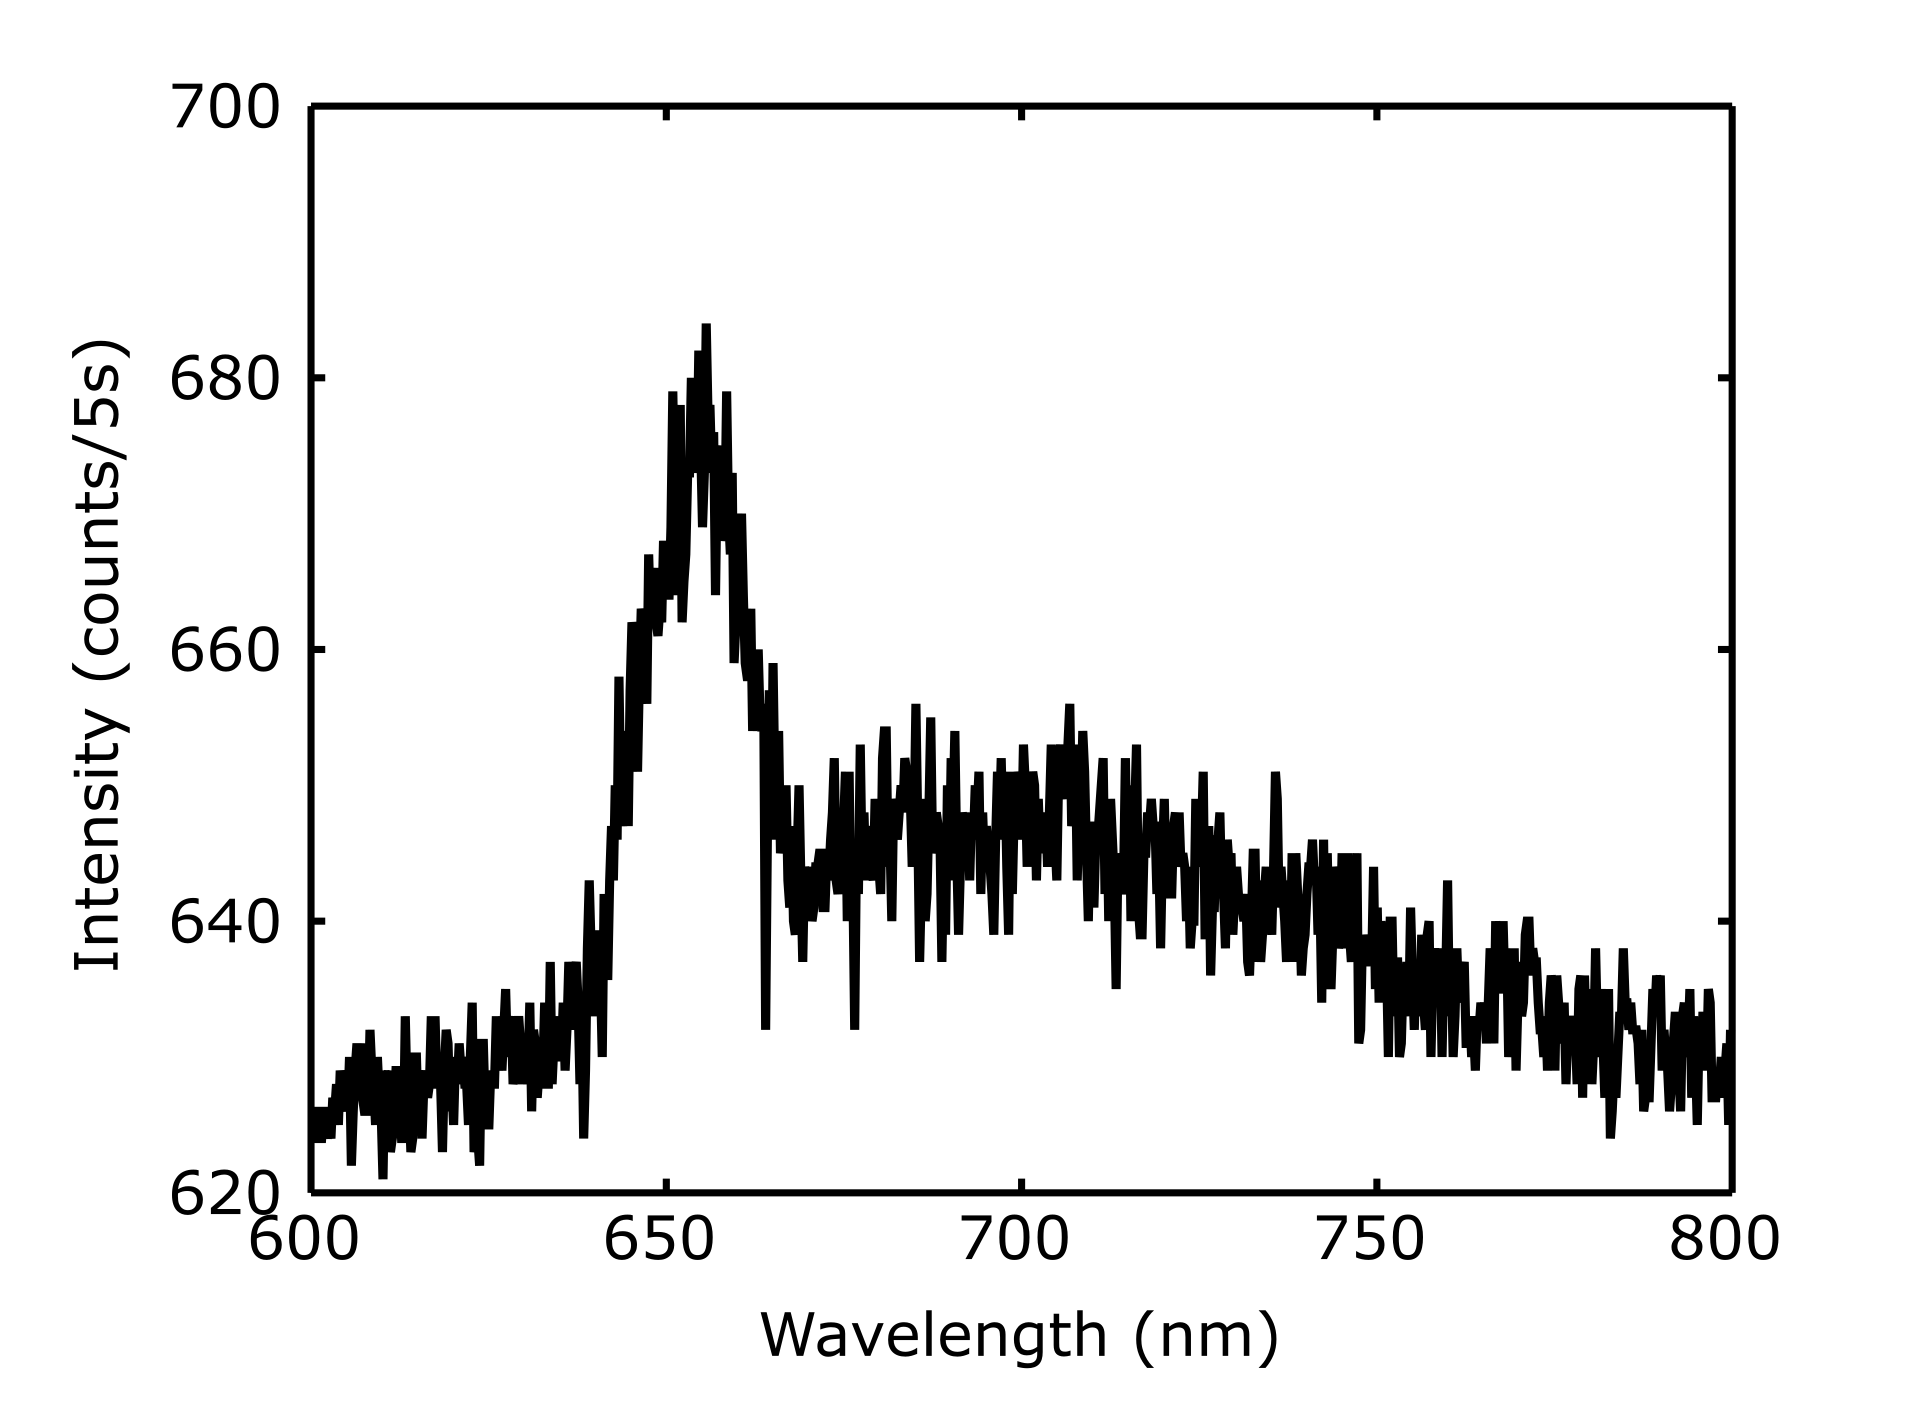
\includegraphics[width=0.95\linewidth]{Figures/04_Supporting/03_Background/background.png}
 \caption{Spectra from the background while exciting with a $532\nm$ laser. The
 peak appearing at $650\nm$ is Raman scattering from water.}
 \label{fig:Background}
\end{figure}

Figure S\ref{fig:Background} shows the typical background when exciting with a
$532\nm$ laser. The peak at $650\nm$ is Raman scattering from water. Normally
this background can be well subtracted from the spectra acquired on particles.
For less intense curves however, it is possible to observe shoulder appearing
at this particular wavelength. We conclude that it is due to a non complete
subtraction of the background. 

\end{document}